% running-simulations.tex
\section{Running simulations}
%
Setting up a simulation is mostly an exercise in writing a text-based 
description of your flow and its bounding geometry.
This \textit{input script} is presented to the preparation program as 
a Python source file, often with the extension ``.py''.
Once you have prepared your flow specification as an input script using your favourite text editor, 
the simulation data is generated by the \texttt{Eilmer3} programs in a number of stages:
\begin{itemize}
\item[1] Create the geometry definition, a grid and the initial flow state.
  For simple to moderately complex geometries, the built-in geometry tools (described later in this manual)
  are adequate.
  For complex geometries, you may find it convenient to import block-structured grids, 
  possibly from a specialized gridding tool such as \texttt{Gridgen} or \texttt{ICEMCFD}.
\item[2] Run the simulation code to produce flow data at subsequent times.
\item[3] Reformat the flow solution data to produce files suitable for a data viewing program such as Paraview or GNU-Plot.
\end{itemize}

\newpage
\subsection{Data preparation (with e3prep.py)}
Create the geometry definition and a grid with the command\\
         \texttt{\$ e3prep.py --job=\textit{job} --do-svg }\\ \index{e3prep.py!using}\index{preparation}
         \vspace{0.25cm} \\
         \centerline{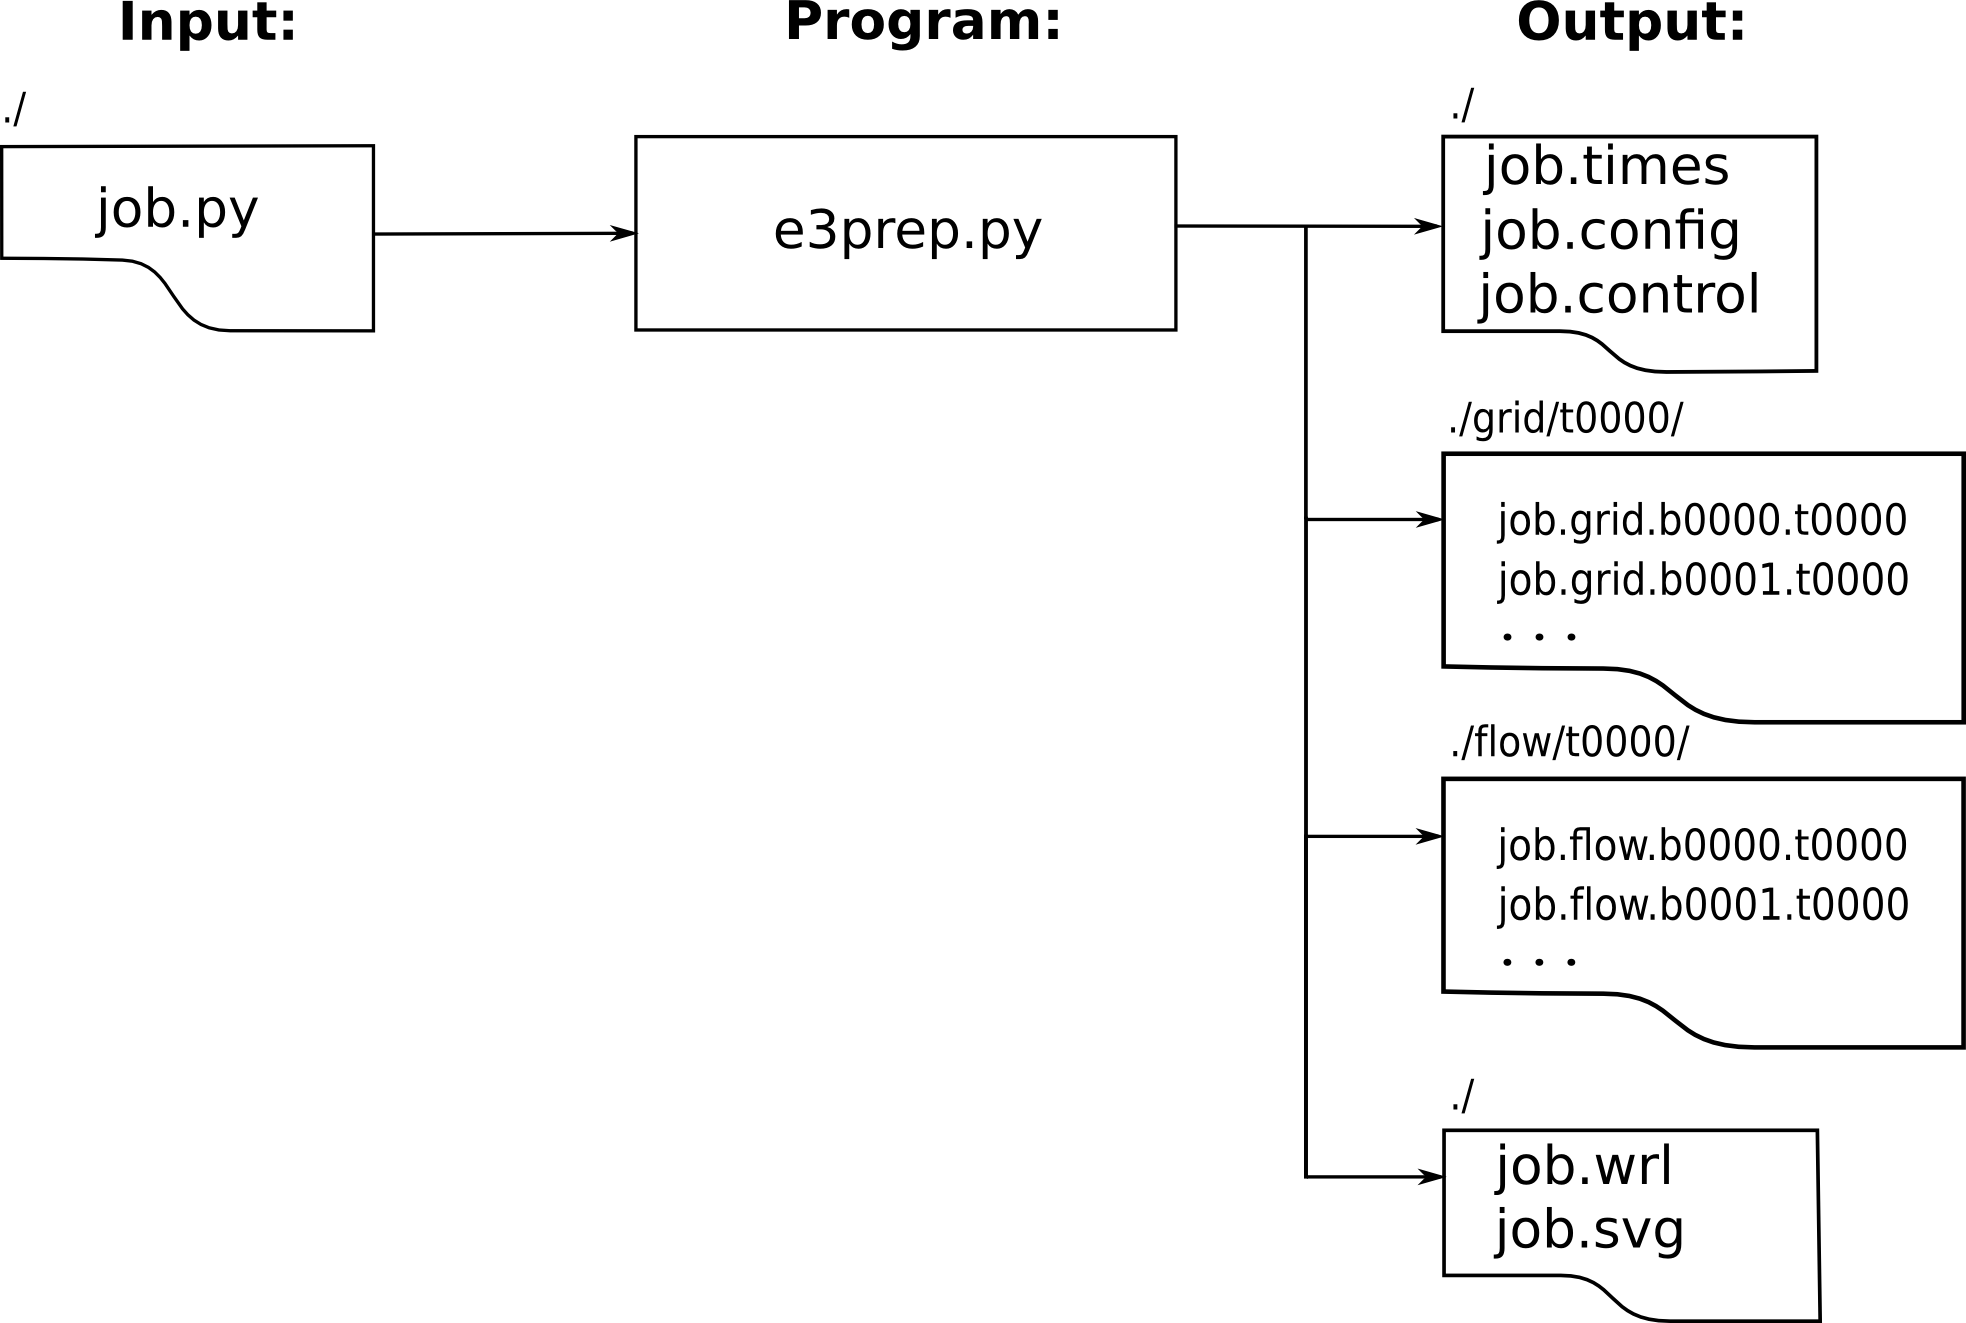
\includegraphics[width=0.7\textwidth]{figs/preparation.png}}\\
         The italics word \textit{job} in the command should be replaced 
         by whatever job name that you have chosen.
         That name is then used as a base to derive specific names for each of
         the files associated with the simulation.
         At a minimum, you have an input script called \textit{job}\texttt{.py} 
         with the \texttt{.py} extension, indicating that the script is written in Python.
         The files from the preparation stage are:
         \begin{itemize}
           \item \textit{job}\texttt{.config}: \index{config file}
             A database of configuration parameters in INI format.
             Parameters are specified, one per line, as \textit{parameter-name = value}.
             A hierarchical structure is given to the set of parameters via
             named subsections in the file.
             Although you would probably never assemble one of these parameter files
             from scratch manually, it is sometimes convenient to alter a value or two and rerun
             a simulation without invoking \texttt{e3prep.py}.
           \item \textit{job}\texttt{.control}: \index{control file}
             A small database of parameters to control the time-stepping, the final time,
             and the intervals between writing of solutions and history data.
             The content of this file is also in INI format and it is parsed at the
             start of every time step.
             This way, a user can alter the simulation behaviour (by editing this file)
             without having to restart the simulation.
             To stop a simulation cleanly, set the \texttt{halt\_now} entry to 1.\index{halting a simulation}
             Other control parameters are marked with \ddag~ in Section\,\ref{sec:sim-control-parameters}.
           \item  \textit{job}\texttt{.times}:
             A mapping of time stamps to actual times at which the simulation
             data was written.
             After the preparation stage, there should be only the zero-time entry.
           \item \textit{job}\texttt{.svg} or \textit{job}\texttt{.wrl}: \index{SVG} \index{VRML}
             Sometimes it is convenient to see a graphical representation of the flow domain 
             and boundary conditions.
             These options produce a SVG or VRML rendering of the block boundaries 
             and the boundary-condition labels.
             The \texttt{--do-svg} will invoke the rendering of two-dimensional blocks
             to a scalable-vector-graphics file while \texttt{--do-vrml} will render 
             three-dimensional blocks to a virtual-reality-modeling-language file.
             For two-dimensional simulations, the SVG file can be edited in a program such as \texttt{Inkscape}
             (\url{http://www.inkscape.org})
             and the result used as part of your documentation for a particular simulation.
           \item \textit{job}\texttt{.grid.b0000.t0000}, \textit{job}\texttt{.grid.b0001.t0000} :
             The grid of finite-volume cells, 
             one file for each block that defines part of the flow domain.
             The grids are written as plain text files in a relatively simple format.
             The spatial coordinates for points within each file are
             associated with cell vertices of the structured grid.\footnote{Note that, in recent versions of the programs, 
             the grid and flow files are written to subdirectories within the job directory.}
           \item one flow-data file for each block:
             \textit{job}\texttt{.flow.b0000.t0000}, \textit{job}\texttt{.flow.b0001.t0000}, ...
             containing the initial flow state within each of the finite-volume cells.
             Look at the first couple of lines of a flow file to see what data elements are written for each cell.
             Variable names appear on the second line and units are \texttt{SI}.
         \end{itemize}
         Note that the grid and flow data files are written to subdirectories of the same names.
         The grid is written once (at time zero, subdirectory \texttt{grid/t0000/}) and 
         the flow files are written to a new subdirectory (\texttt{flow/tnnnn/}) at each output time.
         This is to keep the main job directory clean and to allow easy copying or moving of 
         individual solution times.
         Also, these files are stored in ``gzip'' format with a ``.gz'' extension by default.\index{gzip}

\newpage
\subsection{Running the simulation (with e3shared.exe)} 
Run the simulation code to produce flow data at subsequent times.\footnote{If the simulation
finishes too quickly (possibly without taking any steps at all),
it may be that the initial time step size is too large and the calculation is unstable.
One symptom of this is that the final value for \texttt{dt} is reported as being
the excessively large value of \texttt{1e+6} seconds.
Choose a suitably small value and try again.}\\ \index{e3shared.exe!running a simulation}
         \texttt{\$ e3shared.exe --job=\textit{job} --run}\\
         \vspace{0.25cm} \\
         \centerline{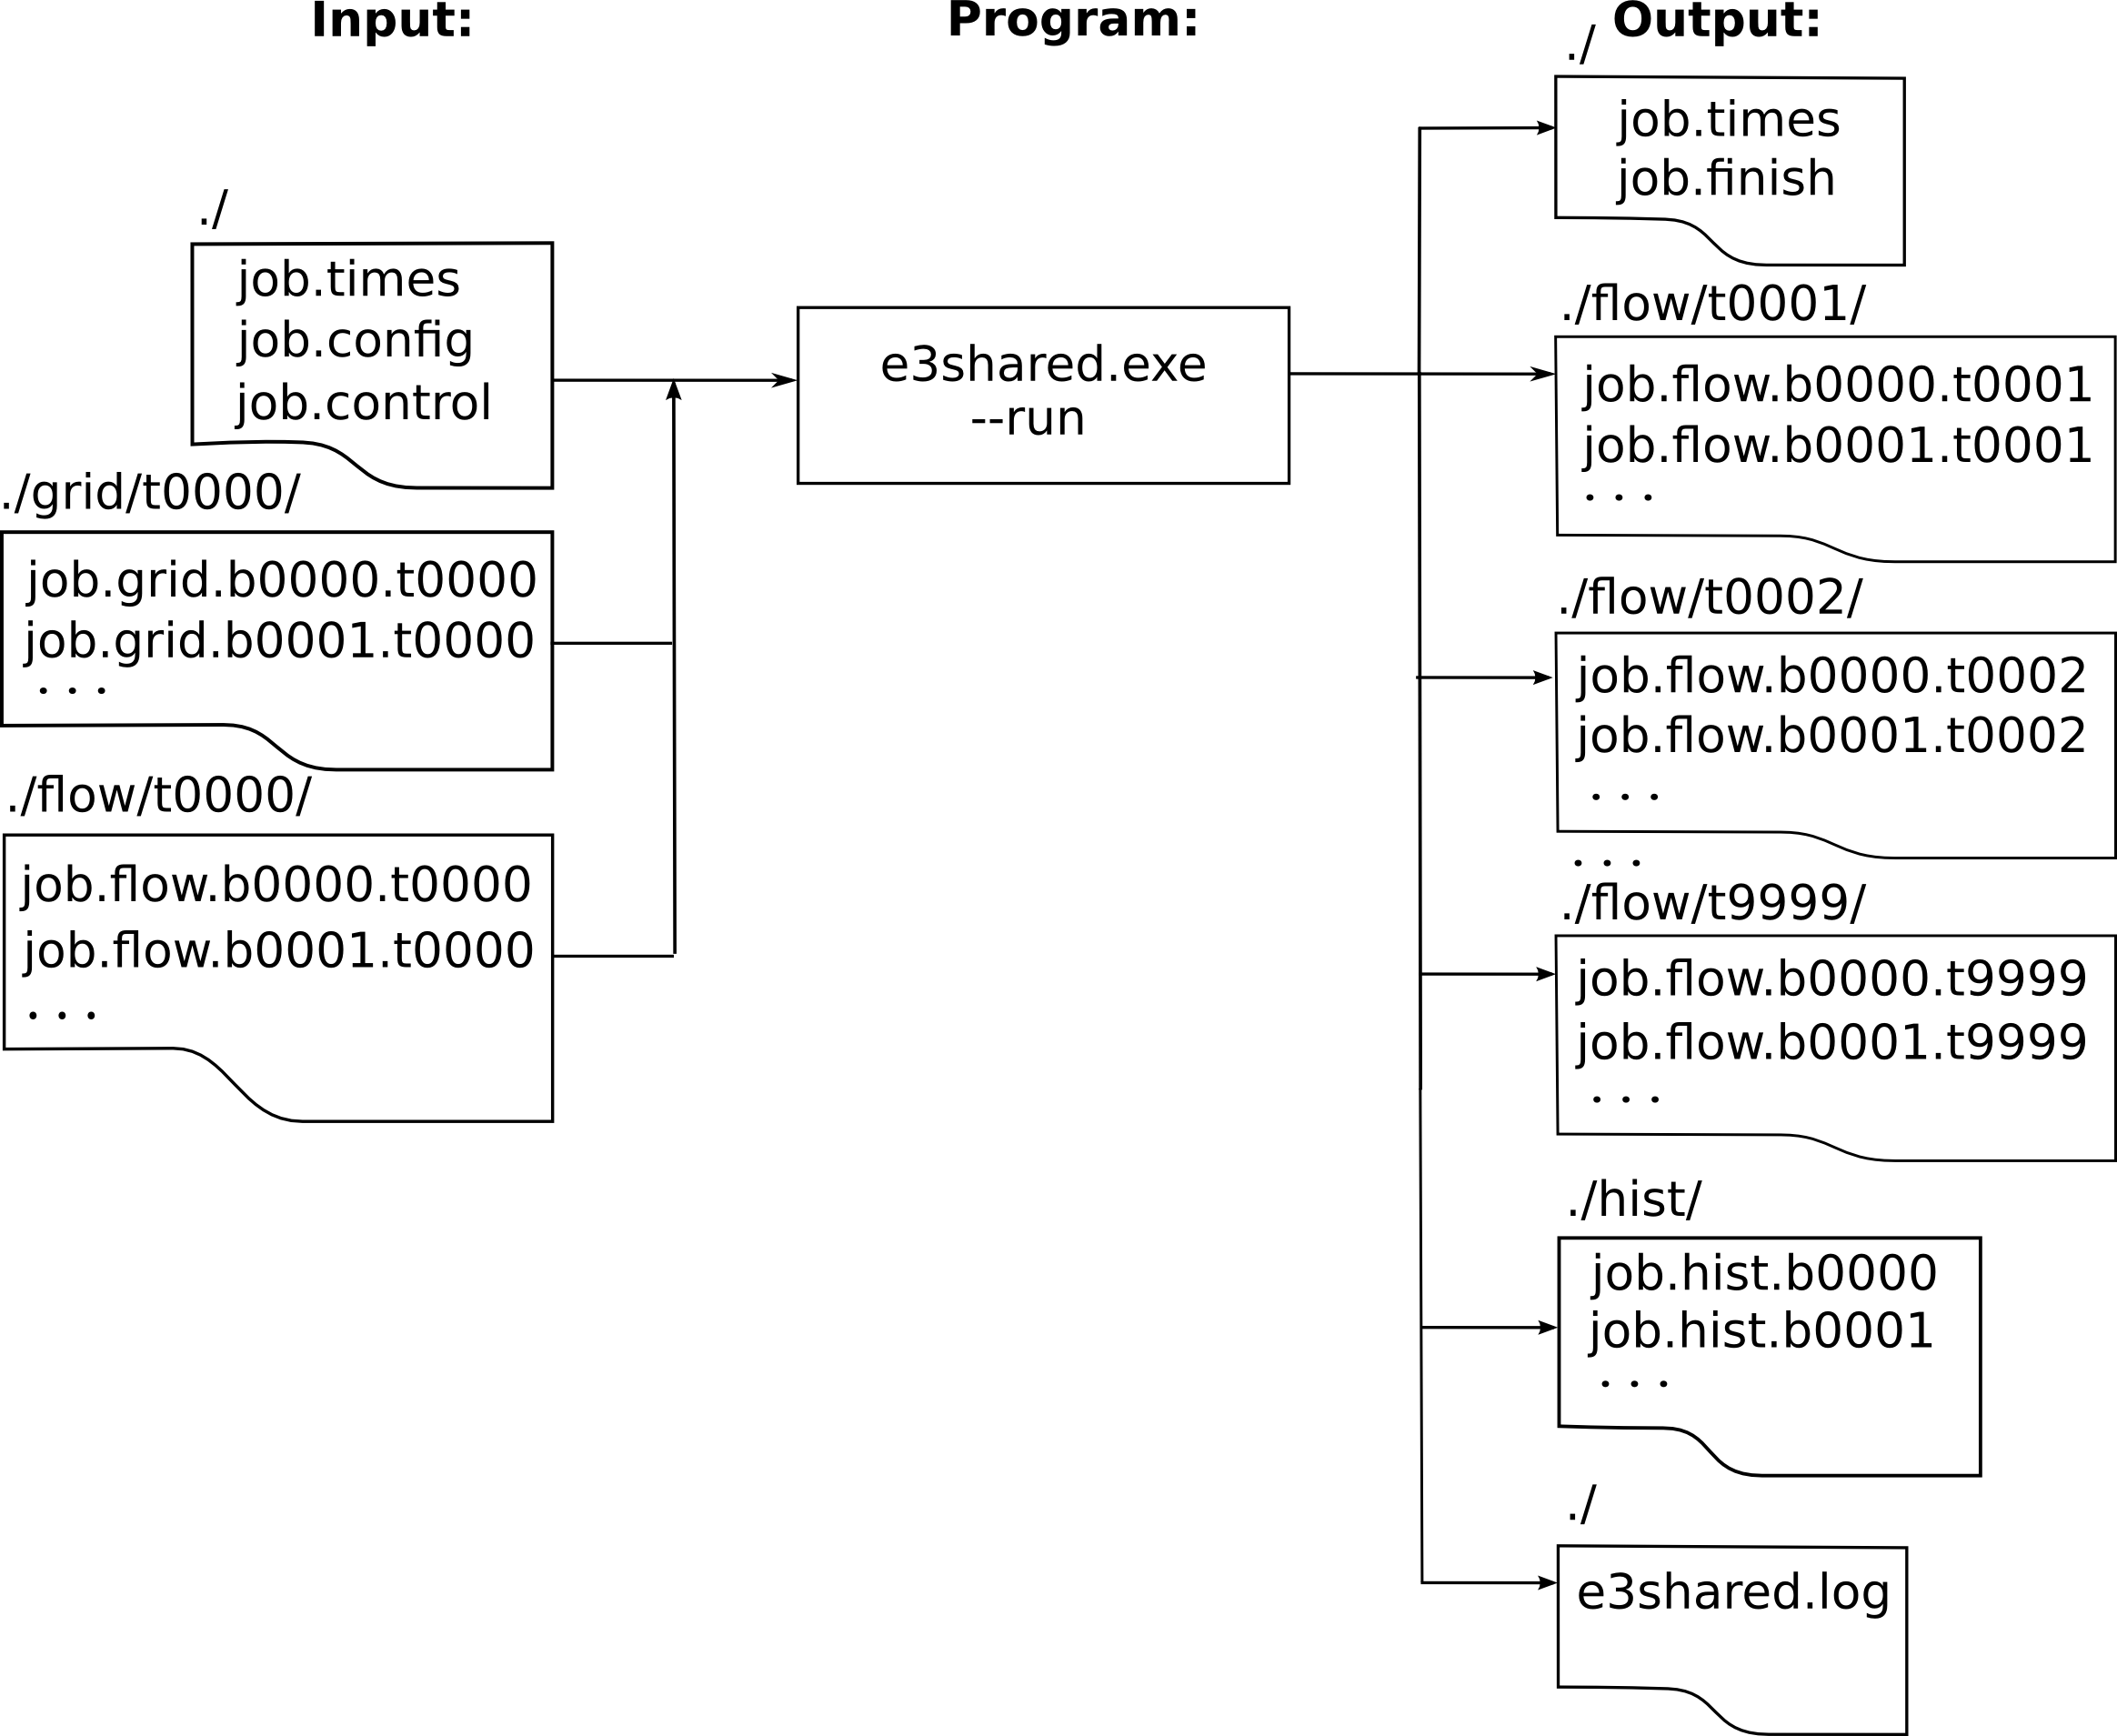
\includegraphics[width=0.7\textwidth]{figs/running-sim.png}}\\
         The output files are:
         \begin{itemize}
           \item \textit{job}\texttt{.flow.b}\textit{nnnn}\texttt{.t}\textit{mmmm}:
             The flow data for all cells at the times requested.
             As the simulation proceeds, whole-field solutions are written
             to new files with \textit{nnnn} representing the block number and
             \textit{mmmm} representing a time stamp.
             Look up the \textit{job}\texttt{.times} file to see what time values
             belong to each time stamp (or tindx).
             Just as for the grid files, each flow solution file is written 
             as a plain text file with a simple layout, not too different from 
             the Tecplot point-format for a structured-block grid.
             In these files, the spatial coordinates of points within the file are
             associated with the cell centres.
           \item  \textit{job}\texttt{.hist.b}\textit{nnnn}: \index{history location}
             Data at particular ``history locations'' and at times requested.
             This data is typically used to simulate the signals recorded by pressure 
             and heat-transfer sensors mounted on model surfaces.
             When restarting a simulation, the program will append to existing history files 
             rather than clobbering them.
             Note that, if you are running a simulation from the start multiple times, 
             you will need to manually remove the history files before each run.  
             The command \texttt{``rm -r ./hist/''} should do the job.
           \item  \textit{job}\texttt{.times}: \index{times file}
             A mapping of time stamps to actual times at which the simulation
             data was written.
             The main simulation appends lines to this file.
             This file may assist when automating some of the postprocessing operations.
           \item  \textit{job}\texttt{.finish}: \index{finish file}
             An INI-format file giving some information about the time-stepping parameters
             at the end of the simulation.
             These may be useful for starting a follow-on simulation.
         \end{itemize}

\medskip
For viscous simulations, surface heat flux and cell Reynolds number files are also written to the subdirectory \texttt{heat}.
See the \texttt{--heat-flux-list} option in Section\,\ref{sec:e3post} for a hint at how to extract the data and then
have a look in the data files to see what specific data has been captured. 

\subsection{Running the simulation in parallel (e3mpi.exe)}
%
One can build and run the distributed-memory version of the program, 
\texttt{e3mpi.exe}\index{e3mpi.exe}, on computers with 
the MPI (Message Passing Interface) library\footnote{See, for example, \url{http://www.open-mpi.org/}.} 
and runtime environment.
The notes in Appendix\,\ref{getting-started-file} show how to build and run 
the Eilmer3 executable for OpenMPI.\footnote{These notes are also available in HTML form at the URL
\url{http://www.mech.uq.edu.au/cfcfd/}.}
To run Eilmer3 across multiple processors\index{e3mpi.exe!running a simulation}
on a local machine use the following command\\
\texttt{\$ mpirun -np \textit{n} e3mpi.exe --job=name --run}\\
where \textit{n} is the number of MPI processes to use.
Note that when running the program with these options,
one MPI process is assigned to each block; 
the number of MPI processes \emph{must} match the number of blocks in the simulation.
Each of these MPI processes is a separate program and you may run more than one per core 
or physical processor, however, if you want the shortest calculation time and you had lots of cores,
you would probably run one per core.
For simulations with many blocks, it is sometimes possible to achieve a better balance of
computational load by assigning more than one block to a process.
This is can be done with Eilmer3 by building a mapping file of blocks to MPI processes
(using the \texttt{e3loadbalance.py} program), and then running \texttt{e3mpi.exe} with
the \texttt{--mpimap=} option.
The details of using Eilmer3 in this way are described in Appendix~\ref{app:load-balance}. 

\subsection{Running a radiation transport calculation (e3rad.exe)}
% 
The user can build and run the shared-memory version of the radiation transport solver,
\texttt{e3rad.exe}\index{e3rad.exe}, on computers with the OpenMP API.
The notes in Appendix\,\ref{getting-started-file} show how to build and run 
the Eilmer3 radiation transport solver executable for OpenMP.\footnote{These notes are
 also available in HTML form at the URL \url{http://www.mech.uq.edu.au/cfcfd/}.}


\subsection{Restarting a simulation}\index{restarting a simulation}
%
By default, the simulation program picks up the flow solution for \texttt{tindx} equal to 0 but
it can be told to pick up any other \texttt{tindx} snapshot.
To pick up a solution and continue, it is probably best to do a little house-keeping with the command\\
\texttt{\$ e3post.py --job=name --prepare-restart}\\
This renames the 9999 flow files and tidies up the \textit{job}\texttt{.times} file to reflect the changes.
Then you should edit the \textit{job}\texttt{.control} file and change the parameters \texttt{dt}
\texttt{max\_time} and \texttt{max\_steps} to suitable values.
Do \underline{not} run \texttt{e3prep.py} again, else it will write all over 
your newly edited \textit{job}\texttt{.control} file.
At this point, you should be ready to run the main simulation program again.
Remember to supply the relevant \texttt{tindx} value on the command line for your restart.
For example:\\
\texttt{\$ e3shared.exe --job=name --tindx=5 --run}

\medskip
Also, with restarts, be careful that you have consistent modelling requirements and settings.
Restarting a laminar simulation as a turbulent simulation with the $k-\omega$ model would lead
to inconsistent data.
It may be better to start a new job and use \texttt{ExistingSolution} objects\footnote{We need to make \texttt{ExistingSolution} smart enough to fill in missing values.} (see Section\,\ref{sec:ExistingSolution}) to pick up the old data. 

\newpage
\subsection{Postprocessing (with e3post.py)}\index{postprocessing} 
\label{sec:e3post}
%
Postprocessing of the simulation data is the most unstructured of the simulation activities.
We provide a postprocessing program, \texttt{e3post.py} that has the basic capabilities of picking up 
the simulation data and writing flow field files in formats suitable for 
\texttt{Paraview}, \texttt{Visit}, \texttt{Tecplot}, the venerable \texttt{Plot3D} or 
\texttt{gnuplot}\footnote{See the web sites  \url{http://www.paraview.org}, \url{https://wci.llnl.gov/codes/visit/},
\url{http://www.tecplot.com}, \url{http://people.nas.nasa.gov/\~rogers/plot3d/intro.html} and \url{http://www.gnuplot.info}}.
\vspace{0.25cm} \\
\centerline{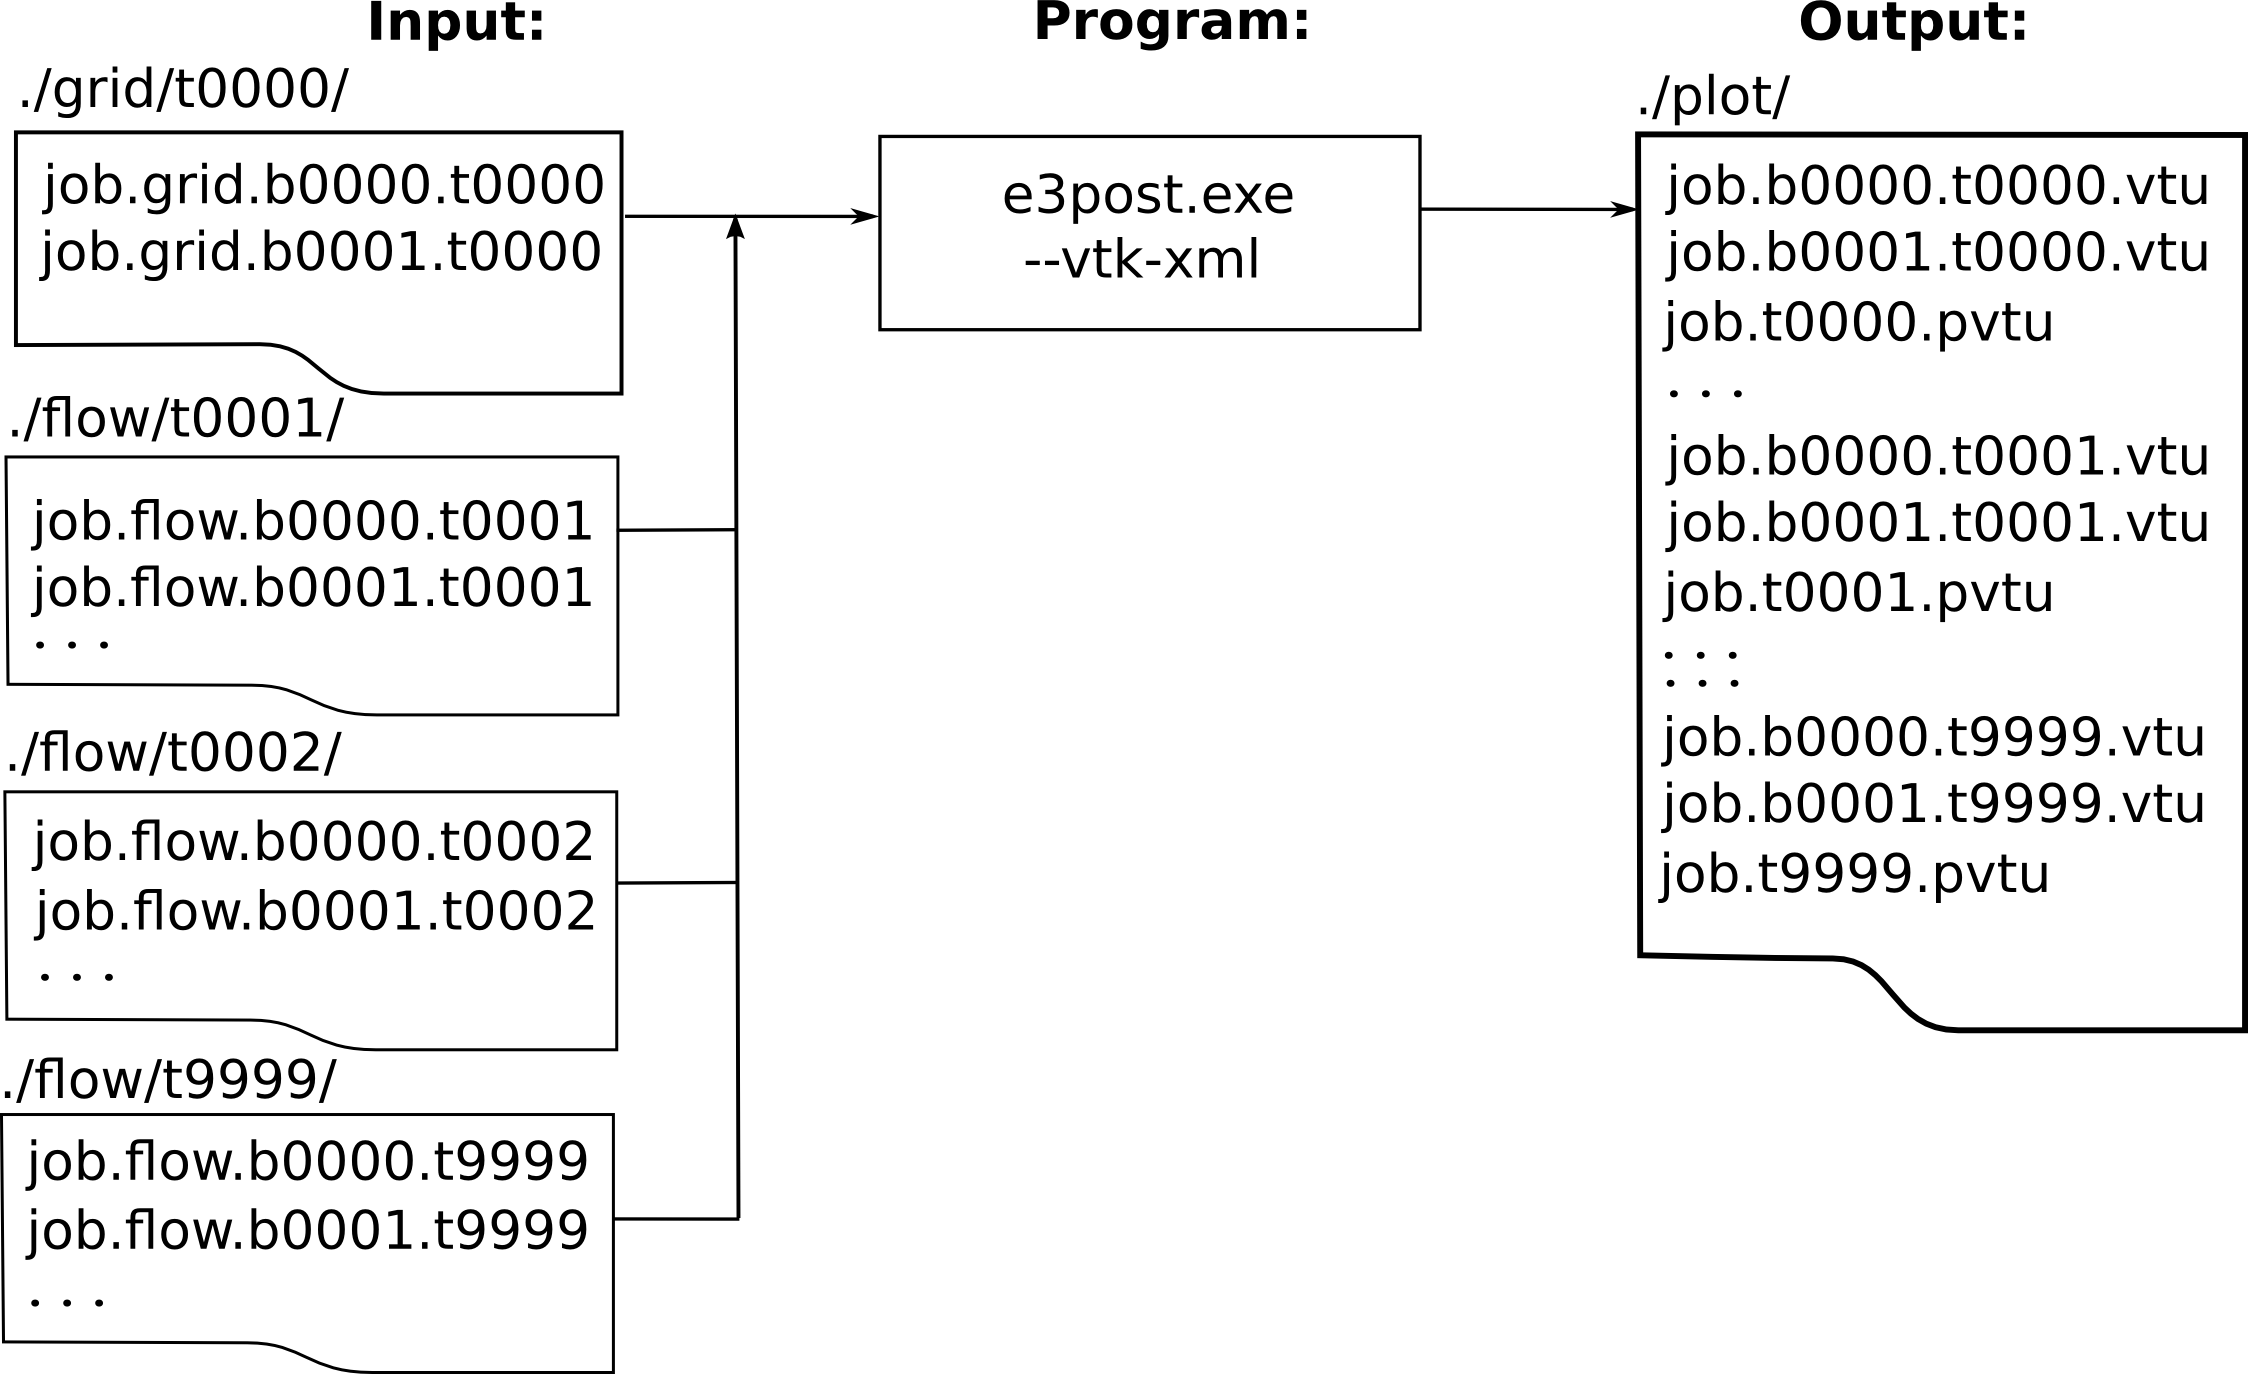
\includegraphics[width=0.7\textwidth]{figs/post-process.png}}\\

\medskip
To reformat the flow solution data into one unstructured grid
containing all of the flow data for the domain and write this data in a format suitable
for \texttt{Paraview} or \texttt{Visit}, use the command:\\
\texttt{\$ e3post.py --job=\textit{job} --vtk-xml --tindx=all}\\ \index{e3post.py!using}

\medskip
The postprocessing program (\texttt{e3\_post.py}) started as a fairly simple script that picked up solution data
and reformatted it for plotting, however, it has continued to sprout features and has become a bit 
complex to describe.
To see its command-line options, just run it without any options at all.
It should then print a \textit{usage} message which provides some hints.
As at October 2009, the start of this message is:

\noindent
{\footnotesize
\begin{verbatim}
Begin e3post.py...

Usage: e3post.py [--help] [--job=<jobFileName>] [--tindx=<index|all>]
                 [--zip-files|--no-zip-files]
                 [--vtk-xml] [--tecplot] [--plot3d]
                 [--prepare-restart] [--prepare-fstc-restart]
                 [--put-into-folders]
                 [--ref-function=<python-script>]
                 [--report-norms]
                 [--per-block-norm-list="jb,var-name,norm-name;..."
                 [--global-norm-list="var-name,norm-name;..."
                 [--compare-job=<jobFileName> [--compare-tindx=<index>]]
                 [--output-file=<profile-data-file>]
                 [--slice-list="blk-range,i-range,j-range,k-range;..."]
                 [--slice-at-point="blk-range,index-pair,x,y,z;..."]
                 [--slice-along-line="x0,y0,z0,x1,y1,z1,N"]
                 [--surface-list="blk,surface-name;..."]
                 [--add-pitot-p] [--add-total-p] [--add-mach] [--add-total-enthalpy]
                 [--add-molef --gmodel-file="gas-model.lua"]
                 [--probe="x,y,z;..."]
                 [--heat-flux-list="blk-range,surf-range,i-range,j-range,k-range;..."]
                 [--omegaz="[omegaz0,omegaz1,...]"]
                 [--tangent-slab-list="blk-range,i-range,j-range,k-range;..."]
\end{verbatim}
} % end of \footnotesize

\noindent
The options can be combined in fairly complex ways; some experimentation on the part of the user
may be required to get the desired effect.
\begin{itemize}
  \item \texttt{--help} just prints the usage message.  No other options are relevant.
  \item \texttt{--job=<jobFileName>} specifies the root name of the solution files
  \item \texttt{--tindx=<index|all} You may pick up one solution time via its index or you may
     specify all solution times via the keyword ``\texttt{all}''.
  \item \texttt{--zip-files|--no-zip-files} The default behaviour is to use gzipped files for the
     grid and flow data files, however, earlier version of the code used plain text files that were not zipped.
  \item \texttt{--vtk-xml} The XML format for the Visualization Tool Kit (VTK) is readable by both \texttt{Paraview}
     and \texttt{Visit}.
  \item \texttt{--tecplot} This produces an ASCII file that can be read by \texttt{Tecplot}.
  \item \texttt{--plot3d} This is also an ASCII format file that many visualization and flow simulation
     packages read and write.
     Two grid files are generated.  The first, with \texttt{.grd} extension, 
     is the true grid as used by the simulation with mesh location at the nodes.  
     The second, with extension \texttt{.g}, has cell-centred values and accompanies 
     the cell-centred values in the \texttt{.f} file.
  \item \texttt{--prepare-restart} does some house-keeping in the data files so that a simulation 
     may be restarted cleanly.  
     This is mainly dealing with the \texttt{9999} file and adjusting the \texttt{.times} file.
  \item \texttt{--put-into-folders} puts an old solution (which has its files all sitting in the current directory)
     into the current directory structure where the grid, flow and plot files have their own subdirectories.
  \item \texttt{--ref-function=<python-script>} compares the flow solution with a supplied Python function.
     The difference is output.
  \item \texttt{--report-norms} returns a dictionary of norms for all of the flow variables.
    The available norms are \texttt{L1}, \texttt{L2}, and \texttt{Linf} (maximum magnitude).
  \item \texttt{--per-block-norm-list="jb,var-name,norm-name;..."} returns the specified norms 
     for particular variables and blocks.  Sometimes just a little bit of information is required.
  \item \texttt{--global-norm-list="var-name,norm-name;..."} returns the specified norms,
     computed over the whole flow domain.
  \item \texttt{--compare-job=<jobFileName> [--compare-tindx=<index>]} compares one flow data set with another.
     The difference is output.  This option combined with the computation of norms is a convenient way to check
     convergence in of a simulation.
  \item \texttt{--output-file=<profile-data-file>} specifies the name of a file in which to dump the requested data.
     This naming option is relevant to the various slice options and also to the the surface-list option where
     where it is used as the root name of the generated VTK files.
     This will allow you to make a number of sliced data sets for plotting.
  \item \texttt{--slice-list="blk-range,i-range,j-range,k-range;..."} allows one to extract subsets of the data.
     A Python-like slicing notation is used in the specification string which should be enclosed in quotes, as shown. 
     Several slices (separated by semicolons) may be specified in the one string.
     Each slice specification consists of 4 indices or index ranges separated by commas.  
     An index is a single integer value and may be negative to indicate counting from the end.
     A value of \texttt{-1} indicates the maximum value.
     An index range may be a colon-separated pair of integers, a colon and one limit 
     or just a colon by itself (to indicate the full range).
     Note that the range limits are inclusive.
     So, for example, to extract the EAST strip of cells from block 0 in a 2D simulation, you would use
     the string \texttt{"0,-1,:,0"}.
  \item \texttt{--slice-at-point="blk-range,index-pair,x,y,z;..."} allows one to extract a slice/plane of data
     through a particular point.
     The index-pair is one of ij, jk or ki.  
     The program sets these indices to zero and searches along the remaining index to find the cell nearest 
     the specified (x,y,z) point.
     Once found, the slice over the index pair is selected for output (by adding it to the slice-list.
     Be aware that, for each block selected, slice-at-point will always select a slice to output, 
     even if it is not very close.
     Again, use quotes to hold the string together as it passed through the shell interpreter.
  \item \texttt{--slice-along-line="x0,y0,z0,x1,y1,z1,N"} generates a list of \texttt{N} sampled points between
     the specified end points.
     The sampled data is taken from the nearest cell-centre for eash sample point.
     No higher-order interpolation is done.
  \item \texttt{--surface-list="blk,surface-name;..."} extracts a set of surfaces from the full flow field and 
     writes them as VTK files.  
     Sometimes we want convenient access to the bounding surfaces of the blocks.
     Use \texttt{NORTH}, \texttt{EAST}, \texttt{SOUTH}, \texttt{WEST}, \texttt{TOP} and \texttt{BOTTOM} 
     as the surface names.
  \item \texttt{--add-pitot-p}, \texttt{--add-total-p}, \texttt{--add-mach} and \texttt{--add-total-enthalpy} add the
     named variable to the plotting data set, either for the full field (VTK, Tecplot and Plot3D format) or for sliced data.
     These flow variables are not in the Eilmer3 native flow solution file and must be reconstructed by \texttt{e3post.py}.
  \item \texttt{--probe="x,y,z;..."} reports the sampled data for the specified points.
     The selected data is written in gnuplot format.
  \item \texttt{--heat-flux-list="blk-range,surf-range,i-range,j-range,k-range;..."}\,\footnote{Dan Potter's heat flux code writes
     the heat fluxes for a collection of surfaces.  This was part of his PhD work.} extracts surface heat flux and cell Reynolds number data.
     The syntax is the same as the \texttt{--slice-list} option except that the second argument is the boundary index 
     (\texttt{NORTH}, \texttt{SOUTH}, \texttt{WEST}, \texttt{EAST}, \texttt{TOP} or \texttt{BOTTOM}).
     For 2D simulations, the block and boundary indices are sufficient to define the edge, 
     so you can then leave the \texttt{i-range}, \texttt{j-range} and \texttt{k-range} arguments blank.
     For 3D simulations you would need to specify either \texttt{i}, \texttt{j} or \texttt{k} to get a single line of cells.
     For any range, it is sufficient to give just a colon to get the full range.
     For the surface range, the order of the boundary names comes into play with \texttt{NORTH}=0 and \texttt{BOTTOM}=5.
\end{itemize}
Note that you must use double-quotes on some specification strings to prevent the command shell 
from pulling the string apart (or otherwise changing it) before giving it to \texttt{e3post.py}.

\medskip 
Ad hoc postprocessing\index{postprocessing!customized} is possible by picking up the cell-centre flow
data with your own custom postprocessing program written in Python.
Two Python modules (\texttt{e3\_flow.py}\index{module!e3\_flow.py} and \texttt{e3\_grid.py}\index{module!e3\_grid.py}) 
are available for picking up individual blocks of data and storing
selected flow properties in numpy arrays.
Note that three-dimensional arrays are always used, even for two-dimensional simulations
where the k-index has the single value 0.
The examples that make up the bulk of this manual show some of the things that are possible.
Two specific applications of writing a custom postprocessing script are the estimation of 
surface force on the 10$^o$ ramp case (Section \ref{simple-ramp-sec}) and 
finding the location of the bow shock for the finite cylinder simulation.

\subsection{Supervisory GUI}
%
To ease new-comers into the use of the codes, the \texttt{e3console.tcl} program provides
a graphical view of the simulation process.
It provides straight-forward automation of the simple case of running a simulation
from scratch and then reformatting the entire flow-field data for plotting.
Figure\,\ref{e3console-screenshot-fig} shows the state of the GUI just after running the
cone20 simulation.
The Python input file is shown in the top text frame of the main window, 
with the log of the standard output from the simulation shown in the lower text frame.
The tab for the postprocessor is visible in the ``Options'' window.
It indicates that \texttt{e3post.py} will reformat all the flow data into the XML
file format for the VTK plotting library (as used by Paraview).
Also, note the text in the console window which shows the underlying commands that have been used. 

\begin{figure}
 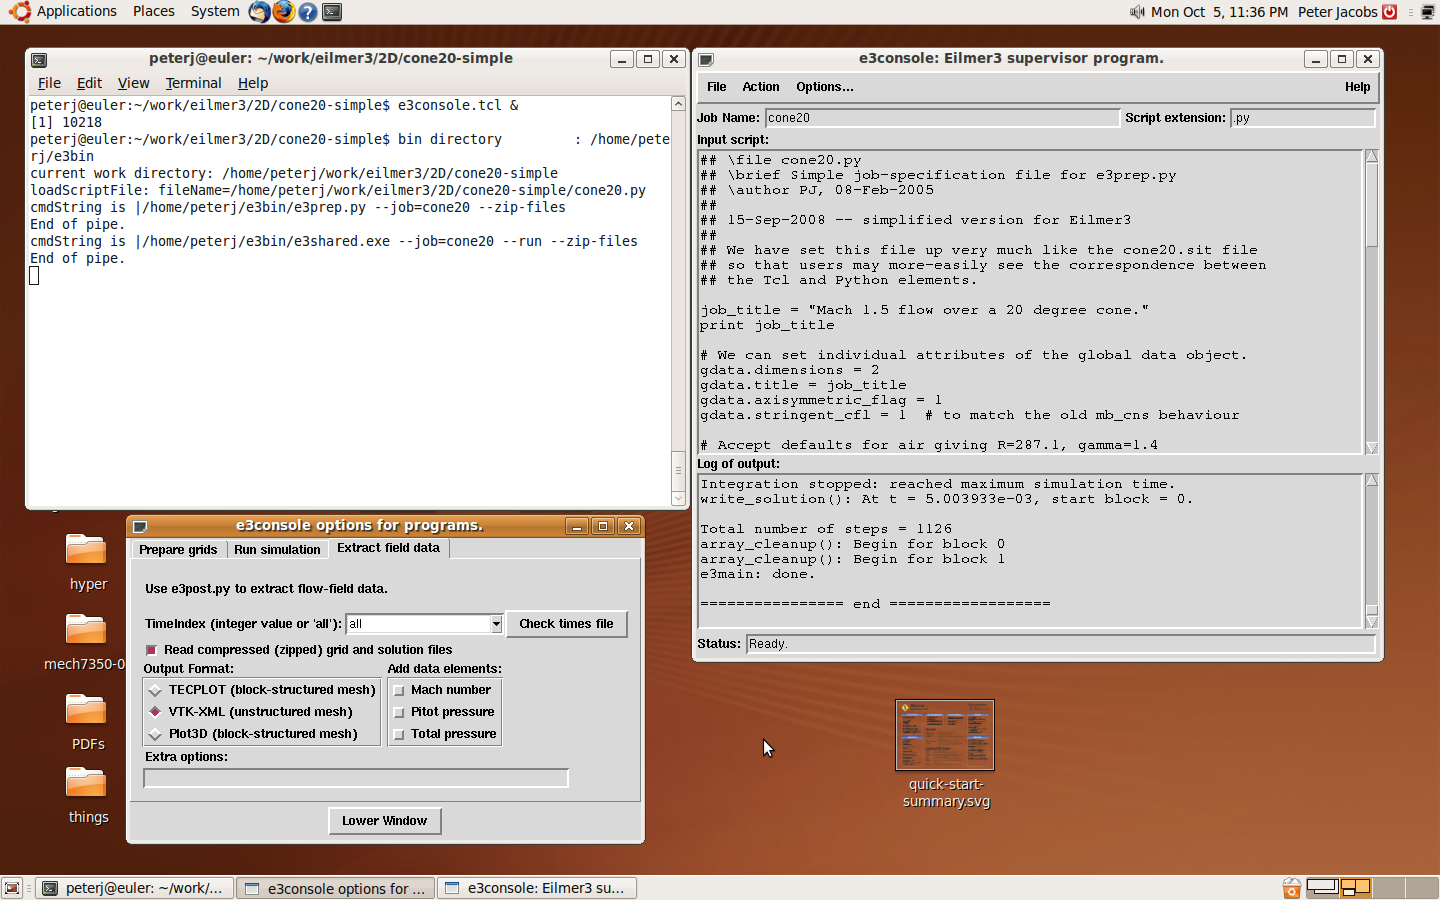
\includegraphics[width=\textwidth]{figs/e3console-screenshot.png}
 \caption{Screen shot of the \texttt{e3console.tcl} GUI running on PJ's workstation.}
 \label{e3console-screenshot-fig}
\end{figure}
